
\chapter{Sentiment Classification}
This chapter describes the experiments done. High level description and
execution of experiments. Detailed descriptions of execution and technical
details in appendix. 

Sections in this chapter are as follows. Manual classifications,
\label{sentiment:manual_classification}, where we see how people classify
tweets. Then we count words with 'Word count classification',
\label{sentiment:word_count_classification}. Expanding with the use of
classifiers in section \label{sentiment:classifier_classification}. A
comparison of the classifiers and associated results can be found in section
\label{sentiment:comparison_results}. And a brief discussion an comments come
last, \label{sentiment:comments_discussion}.

%what is sentiment
Sentiment is described as "an attitude toward something; regard;
opinion."\footnote{ Dictionary.com on Sentiment:
\url{http://dictionary.reference.com/browse/sentiment?s=t}}. The sentiment is the perceived positivity of the message that the user tries to
communicate. Sentiment is in many cases a personal thing, and can change from
person to person or from setting to setting. We think of the sentiment as
conveyed meaning of a message. 

%why do we get it
Some of the motivation for acquiring the sentiment of a tweet or a sentence, is
that we can say something about a persons state of mind and from that predict
behaviour. We want to use the sentiment to make smart decisions later. As an
example of usage it would be ideal to find a correlation between sentiment and
stock exchange, thus making us able to increase revenue with decisions
based on the sentiment. 

%how do we use it
In this thesis we have two main ways of classifying tweets. Word counting and
training a classifier. Both methods require dictionaries of positive and
negative words, \ref{data:dictionaries}. In the classifier we use the dictionary
to extract features from a tweet. And with the word counting we count the
number of positive and negative words. 

\section{Manual Classification}\label{sentiment:manual_classification}
When labeling tweets manually there are a number of factors the complicates the
process. Among them are the quality of the tweet, state of mind, language, and
political affiliation.

The quality of the tweet describes the content in many ways. Does the tweet
contain links or hashtags? Are users mentioned?

State of mind for a person dictates that persons actions in many cases. This
also has an effect on labeling tweets. A positive state of mind classifies more
tweets negative as positive then others.

Political affiliation plays a huge role when labeling the obama tweet set. Do
you like obama? Do you like Romney? Neither? This matters. The tweetset in
itself is pro obama. So while labeling this tweet set we put aside political
influence and looked at the core of the sentiment.

Note that all this happens in the brain during 3 to 60 seconds while reading
the tweet text and is a very rough description of the thoughts happening.
Labeling a tweet follows this algorithm in many ways:

\begin{tabular}{ l p{5cm} p{7cm} }
Step & Thought & Description \\
1 & Have we seen this tweet before? & Skip it or use previous classification. \\
2 & \#Hashtags or links present? & Some hashtags are automatically positive or
negative. Also remove noise such as users and links.\\
3 & Sarcasm? & If sarcasm is present, put up a warning flag saying that it is
the opposite of step 4.\\
4 & Special words? & Find a word that triggers positive or negative
impression.\\
5 & Done & Label tweet as positive or negative.\\
\end{tabular}

\paragraph{Result files}
\hspace{0pt}\\
When classifying with manually we create files with the results. These files
are comma separated files with three fields.
\begin{itemize}
    \item Sentiment: Positive, neutral or negative. Represented by 1, 0 or -1.
    \item Tweet id, if it exists, else 'id'. It is a long number.
    \item The tweet text. In some cases sanitized.
\end{itemize}

\paragraph{Obama tweet set}
\hspace{0pt}\\
When labeling the obama tweet set we found that the tweets present was rather
rubbish. Whether or not the data is representative for twitter in general is
difficult to say. But we observed lots of retweets and political related
content. Tweets favoring obama are positive for poeple who support obama and
negative for supporters of Romney at the same time. So while labeling the
tweets we tried to remove personal political views from the equation, but that
is very difficult in the long run.  

\paragraph{Kiro tweet set}
\hspace{0pt}\\
The kiro tweet set also has a lot of retweets, but they are not use later,
thereby removing the retweet reduced data uniqueness. Also the search terms the
dataset is based on could be broader to increase the spectrum of tweets.  
%

\section{Word count classification}\label{sentiment:word_count_classification}
We describe the classification process and the different parts of it, then we
show the results and discuss the drawbacks of this method. The algorithm does,
simply put, count the positive and negative words. More positive words than
negative means the tweet is positive and vice versa. 

\subsection{Classification}
\paragraph{Polarity} 
\hspace{0pt}\\ 
The polarity of a given tweet is based on the difference in the amount of
positive verses negative words. 

First we calculate the amount of positive words. Then divide that on the total
amount of words. Giving us the percentage of positive words. Then we do the same thing for negative words.

Then we look at the difference between the negative and the positive word
percentage. If the difference is positive we have a positive tweet. And if the
difference is negative we have a negative tweet.

Code wise we get something like this: 
\begin{verbatim}
var positive_words_count
var negative_words_count

positivity = positive_words_count / total_number_words
negativity = negative_words_count / total_number_words

polarity = positivity - negativity

if polarity > 0: 
    tweet is positive
else: 
    tweet is negative
\end{verbatim}

\paragraph{Threshold} 
\hspace{0pt}\\ 
Threshold is the ratio of positive vs negative words that has to be present for a
tweet to be either positive of negative.

The percentage of positive words minus the percentage of negative words gives
the polarity value, or the positivity(how positive a tweet is) of a tweet. 
When actually deciding if a tweet is positive or negative we look at the
polarity value. If the polarity value is above the threshold (polarity >
threshold) the tweet is classified as positive. 

\paragraph{Examples of classification follows:} 
\hspace{0pt}\\ 
Example tweets:
\begin{itemize}
    \item t1 = “good that he was decreasing badly”
    \item t2 = “he was good for increase” 
    \item t3 = “good or bad”
\end{itemize}

Classification of t1:
\begin{itemize}
    \item pos = 1 / 6 = 0.16666
    \item neg = 2 / 6 = 0.33333
    \item polarity = pos - neg = -0.1667
    \item threshold of 0 gives negative classification
    \item threshold of 0.1 gives negative classification
    \item threshold of -0.2 gives positive classification
\end{itemize}

Classification of t2:
\begin{itemize}
    \item pos = 2 / 5 (to av fem ord) = 0.4
    \item neg = 0 / 5 = 0
    \item polarity = pos - neg = 0.4 - 0.0 = 0.4
    \item threshold = 0.4 ⇒ positive
    \item threshold = 0.5 ⇒ negative
    \item threshold = -0.1 ⇒ positive
\end{itemize}

Classification of t3:
\begin{itemize}
    \item pos = 1 / 3 = 0.3333
    \item neg = 1 / 3 = 0.3333
    \item polarity = pos - neg = 0
    \item threshold = 0 ⇒ positive
    \item threshold = 0.1 ⇒ negative
    \item threshold = -0.1 ⇒ positive
\end{itemize}

Further we found the best average threshold value to be 0.1.
From the table under we have the threshold value, and the average
classification accuracy among the 18 entries for each threshold value. 

Average threshold accuracy table:
\hspace{0pt}\\
\begin{tabular}{ c c c c }
Threshold & Accuracy & Threshold & Accuracy \\
- & - & 0.0 & 0.6479 \\
-0.1 & 0.6316 & 0.1 & 0.6516 \\
-0.2 & 0.6161 & 0.2 & 0.6511 \\
-0.3 & 0.6059 & 0.3 & 0.6430 \\
-0.4 & 0.5988 & 0.4 & 0.6305 \\
-0.5 & 0.5888 & 0.5 & 0.6122 \\
-0.6 & 0.5711 & 0.6 & 0.5934 \\
-0.7 & 0.5423 & 0.7 & 0.5712 \\
-0.8 & 0.5083 & 0.8 & 0.5457 \\
-0.9 & 0.4881 & 0.9 & 0.5307 \\
\label{tbl:average_threshold_accuracy}
\end{tabular}

\begin{figure}[htb]
    \centering
    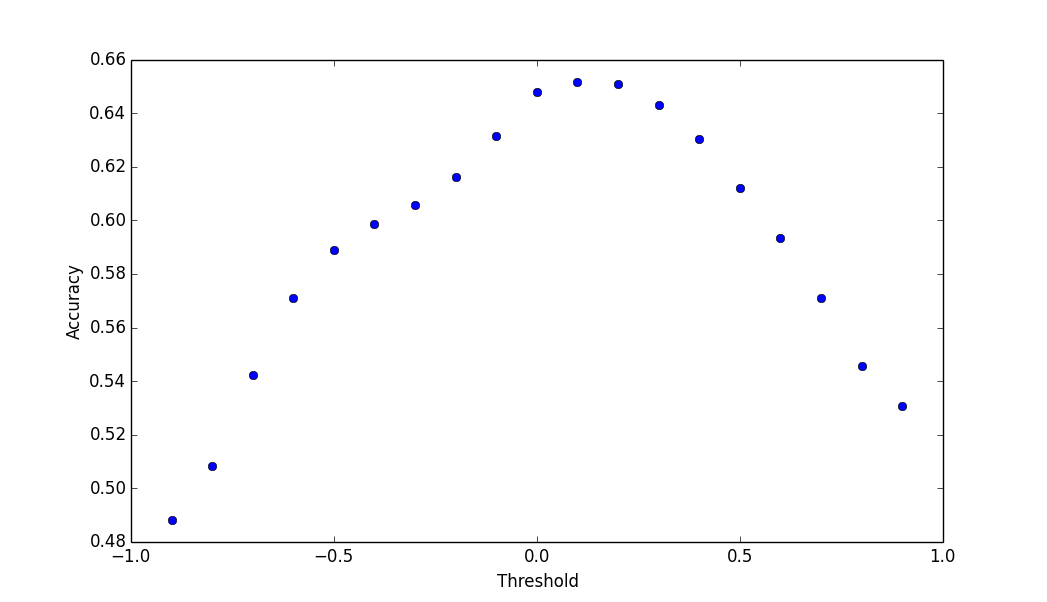
\includegraphics[width=\textwidth]{average_threshold_accuracy.png} 
    \caption{Graph plot of the 'Average threshold accuracy' table.}
    \label{fig:average_threshold_accuracy}
\end{figure}
%

\subsection{Results}
#TODO write results from the classification of the different dictionaries. \\
Dictionaries based on their own dataset naturally scores the best. When cross
classifying we see that the bigram dictionaries score the best. With the
trigram dictionaries nearly as good as the bigram dictionaries.

#TODO write about the variations based on the datasets. \\

\paragraph{Threshold variations}
\hspace{0pt}\\
By varying the threshold we hoped to find an optimal point of which we could
separate tweets based on polarity. From the following
graphs, figure \ref{fig:threshold_graphs}, we can see no clear distinction of
one value being better than the other ones.  

In figure \ref{fig:threshold_graphs} we list the results of the experimentation
with the threshold. Table \ref{tbl:dictionary_to_threshold} lists the
dictionaries and dataset used for which graphs in figure \ref{fig:threshold_graphs}.
'kiro dataset' and 'obama dataset' columns tells which dataset that was
classified in which graph.

\begin{tabular}{ l c c }
\hspace{0pt}\\
Dictionary name and description & kiro dataset & obama dataset \\ 
Obama original, Monogram & 1 & 10 \\
LoughranMcDonald, Monogram & 2 & 11 \\
Combined Obama original and \\ LoughranMcDonald, Monogram & 3 & 12 \\
Kiro, Monogram, self compiled & 4 & 13 \\
Obama, Monogram, self compiled & 5 & 14 \\
Kiro, Bigram, self compiled & 6 & 15 \\
Obama, Bigram, self compiled & 7 & 16 \\
Kiro, Trigram, self compiled & 8 & 17 \\
Obama, Trigram, self compiled & 9 & 18 \\

\label{tbl:dictionary_to_threshold}
\end{tabular}

\begin{figure}[htb]
    \centering
    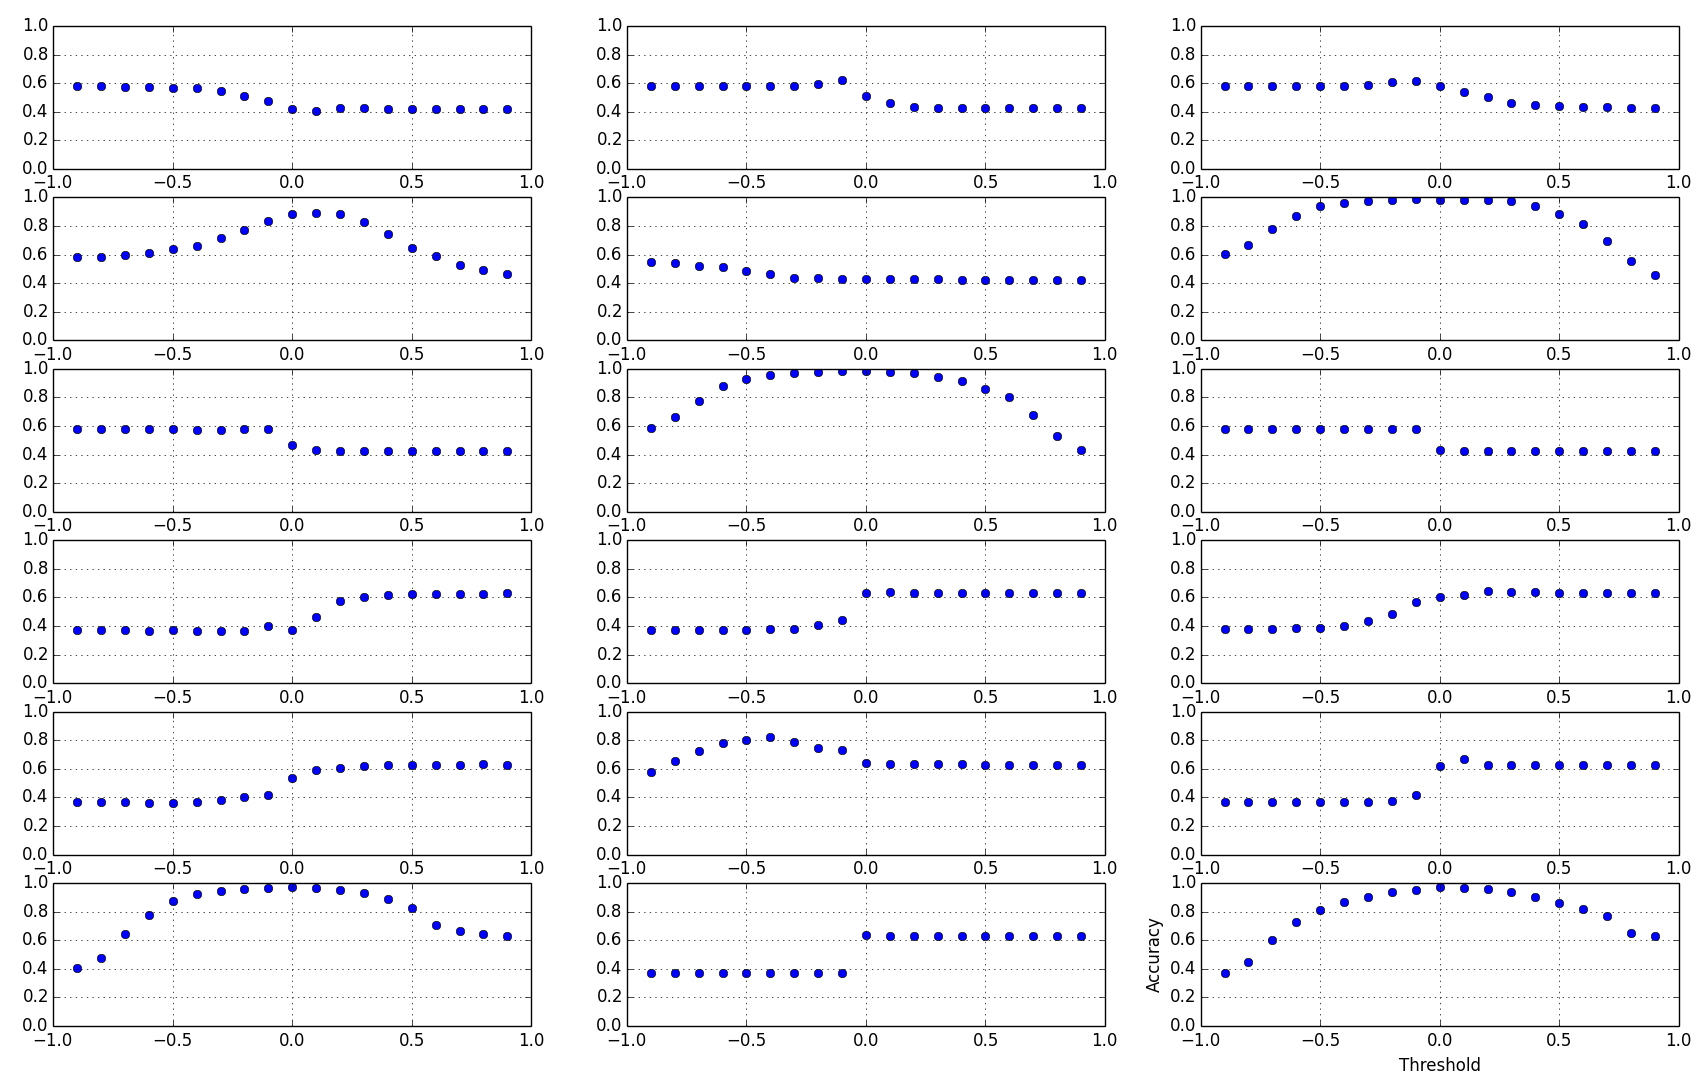
\includegraphics[width=\textwidth]{threshold_graphs.png} 
    \caption{The graphs plot the different variations of threshold. Counting is
columns first; top left is 1, top mid is 7, top right is 13.}
    \label{fig:threshold_graphs}
\end{figure}

\subsection{Drawbacks}
#TODO write about drawbacks.
\paragraph{Dictionaries}
\paragraph{Word positioning}
The dictionaries are based on the manually labeled
tweets, so we can't create bi and tri-grams based on the position of a word in a tweet.
Rather there is no way of automatically decide if a single word is positive or
negative. 

\paragraph{Threshold}
#TODO write how many tweets that end to 0 when threshold is 0.
pos-words == neg-words --> 0 but still the accuracy is quite high.

Although we can se that in line 6 we have very few cases that this happens.
From that we can can conclude that with the right choice of dictionary we don't
have the problem of the threshold value. 

0.0
null cases, 0.0 : 234 of 997
null cases, 0.0 : 543 of 997
null cases, 0.0 : 178 of 997
null cases, 0.0 : 53 of 997
null cases, 0.0 : 14 of 997
null cases, 0.0 : 7 of 997
null cases, 0.0 : 446 of 997
null cases, 0.0 : 28 of 997
null cases, 0.0 : 931 of 997
null cases, 0.0 : 335 of 1365
null cases, 0.0 : 854 of 1365
null cases, 0.0 : 345 of 1365
null cases, 0.0 : 233 of 1365
null cases, 0.0 : 37 of 1365
null cases, 0.0 : 462 of 1365
null cases, 0.0 : 52 of 1365
null cases, 0.0 : 1221 of 1365
null cases, 0.0 : 92 of 1365

\section{With Classifiers}\label{sentiment:classifier_classification}

#TODO write about drawbacks. 

\subsection{SVM}\label{sentiment:svm_classification}
With both datasets.
Using the self compiled monogram dictionaries. 

Results from svm testing. which kernel works best?

\subsection{Naive Bayes}\label{sentiment:naive_bayes_classification}
With both datasets.
Using the self compiled monogram dictionaries. 

Results from testing with different dictionaries. 

\section{Comparison and Results}\label{sentiment:comparison_results}
#TODO highlights of the classifiers \\
#TODO common denominators. commonalities.\\
#TODO comparing the results of the classifiers. \\

\section{Comments and Discussion}\label{sentiment:comments_discussion}

\subsection{}
#TODO Improvements \\

\subsection{Biased Mind}
The datasets of manually labeled tweets are biased based on a persons 
personal opinion and state of mind in the moment of classification.
Therefore we have to keep in mind that all further results are based on the
assumption that everyone agrees on the manual labeling. This is of course a big
potential source of errors to be explored more in \ref{futurework}. 

\subsection{}
#TODO drawbacks \\

\subsection{Conclusions}
#TODO summarize the stuff we have learned shortly. \\

\subsection{}
#TODO future work \\
